%\subsection{Analyses of $e^+e^- \to W^+W^-$} 
%\label{subsec:ew_WWana}

The analysis of four-fermion processes, e.g.\ from $W$-pair production, but also 
 $Z$-boson pairs and single-boson processes, plays a key role in the ILC physics program.  As discussed in Sec.~\ref{subsec:phys_WW}, constraints on triple gauge couplings (TGCs) are an important input to the dim-6 EFT-based interpretation of Higgs precision measurements introduced in Sec.~\ref{subsec:phys_eft}. Prospects for this type of analysis have been intensely studied in full detector simulation (c.f.\ Sec.~\ref{sec:software}), however only at center-of-mass energies of at least 500\,GeV. In this section, we will start out by summarizing these detailed studies, and then proceed to their recent extrapolations to a center-of-mass energy of 250\,GeV.


\subsubsection{Full Simulation Analyses of TGCs}
\label{subsubsec:ew_fullsimww}
The prospects for probing charged TGCs at the ILC have been studied in full, geant4-based simulation of the ILD detector concept at $\sqrt{s}=$500\,GeV~\cite{Marchesini:94888} in the context of the ILD Letter of Intent~\cite{Abe:2010aa} and at $\sqrt{s}=$1\,TeV~\cite{Rosca:2016hcq} as a benchmark for the ILD Detailed Baseline Design (Vol 4 ILC TDR~\cite{Behnke:2013lya}). Both analyses focused on the channel $e^+e^- \to W^+ W^- \to qql\nu$, $l=e, \mu$ and followed a similar, cut-based selection approach. Thereby they exploit the known initial state for a full kinematic reconstruction of both $W$ bosons, under consideration of optional photon radiation collinear to the beam direction.
Neither the case $l=\tau$, nor the fully hadronic mode, nor contributions from single-$W$ production were included at the time. Especially the fully hadronic mode will profit substantially from the recent advances in reconstructing the jet charge with the ILD detector, c.f.\ Sec.~\ref{subsec:ew_ffana}, in order to determine the charges of the $W$ boson candidates.

\begin{figure*}[]
\centerline{
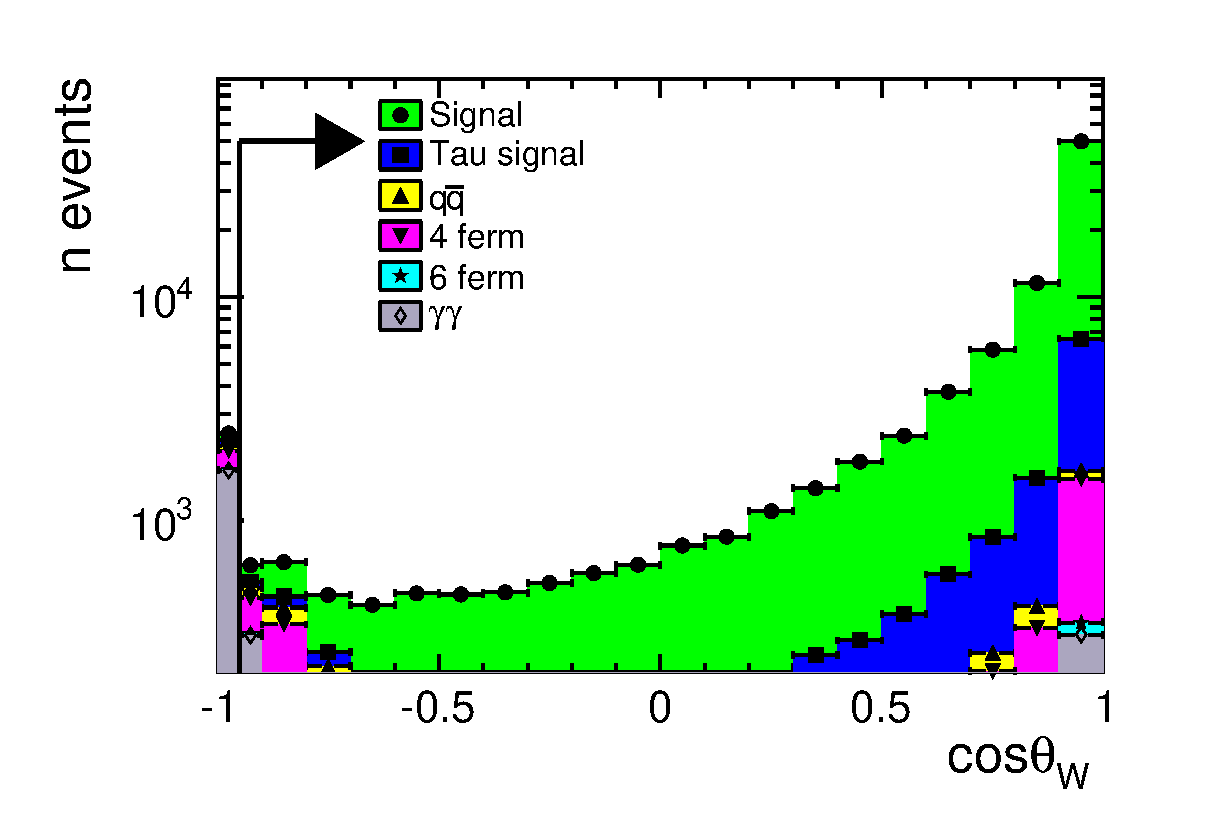
\includegraphics[width=0.5\linewidth]{./chapters/figures/ep+30em-80SUMCosThetaWPRE}
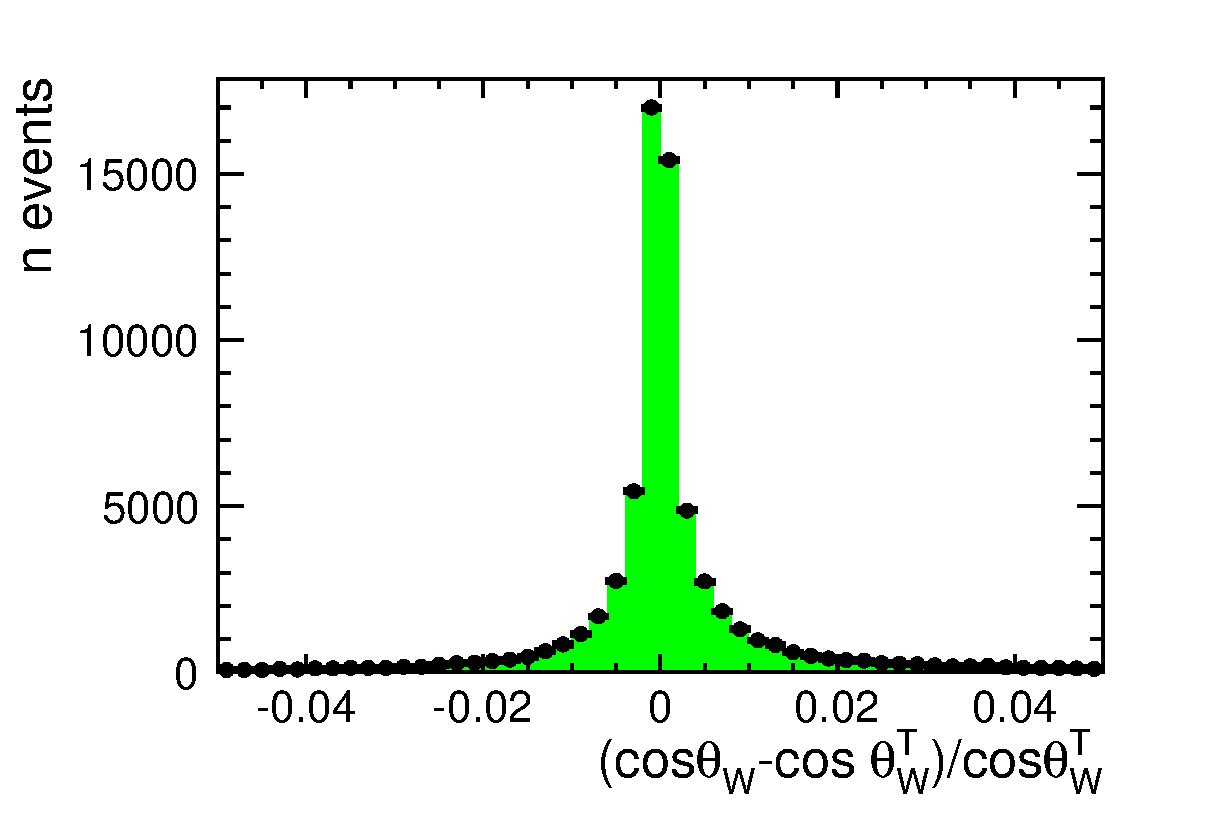
\includegraphics[width=0.5\linewidth]{./chapters/figures/ep+30em-80resolutioncostheta}
}
\caption{Left: Reconstructed polar angle distribution $\cos\theta_{W}$ of the $W^-$ boson candidates for signal and SM background events before the application of the final selection cut $\cos\theta_{W} >$ -0.95. Right: relative deviation of the reconstructed $\cos\theta_{W}$ from the MC truth value $\cos\theta_{W}^\mathrm{T}$. Both from~\cite{Marchesini:94888}.}\label{fig:WW_costheta}
\end{figure*}

Figure~\ref{fig:WW_costheta} shows one of the final observables sensitive to anomalous TGCs,
namely the cosine of the polar angle of the $W^-$ boson, $\cos\theta_{W}$, which is reconstructed from the hadronically decaying $W$ boson. The left part of the figure illustrates the high purity of the selection which ranges between 85\% and 95\%, depending on whether  $WW \to qq\tau \nu$ is considered as background or not. The right panel shows relative deviation of the reconstructed $\cos\theta_{W}$ from MC truth, indicating a resolution of better than 0.5\%.
 
In the 500\,GeV analysis, no pile-up from $\gamma \gamma \to$ low $p_t$ hadrons was considered, which has, at $\sqrt{s}=$500\,GeV, an expectation value of 1.2 events per bunch crossing, c.f.\ Sec.~\ref{sec:software}.
This type of background was considered, however, in the TGC study at 1\,TeV, where its expectation value increases to 4.1 pile-up events per bunch crossing. Figure~\ref{fig:WW_overlayremoval} shows the impact of these pile-up events on the reconstructed hadronic $W$-boson mass without (``Durham'') and with (``Kt'') application of suitable suppression algorithms (see Sec~\ref{subsec:higgs_common} for a detailed description of the algorithm). It can be seen that the residual effect is small even at 1\,TeV, where the number of pile-up events is expected to be nearly four times higher than at 500\,GeV.

\begin{figure}
	\centering
		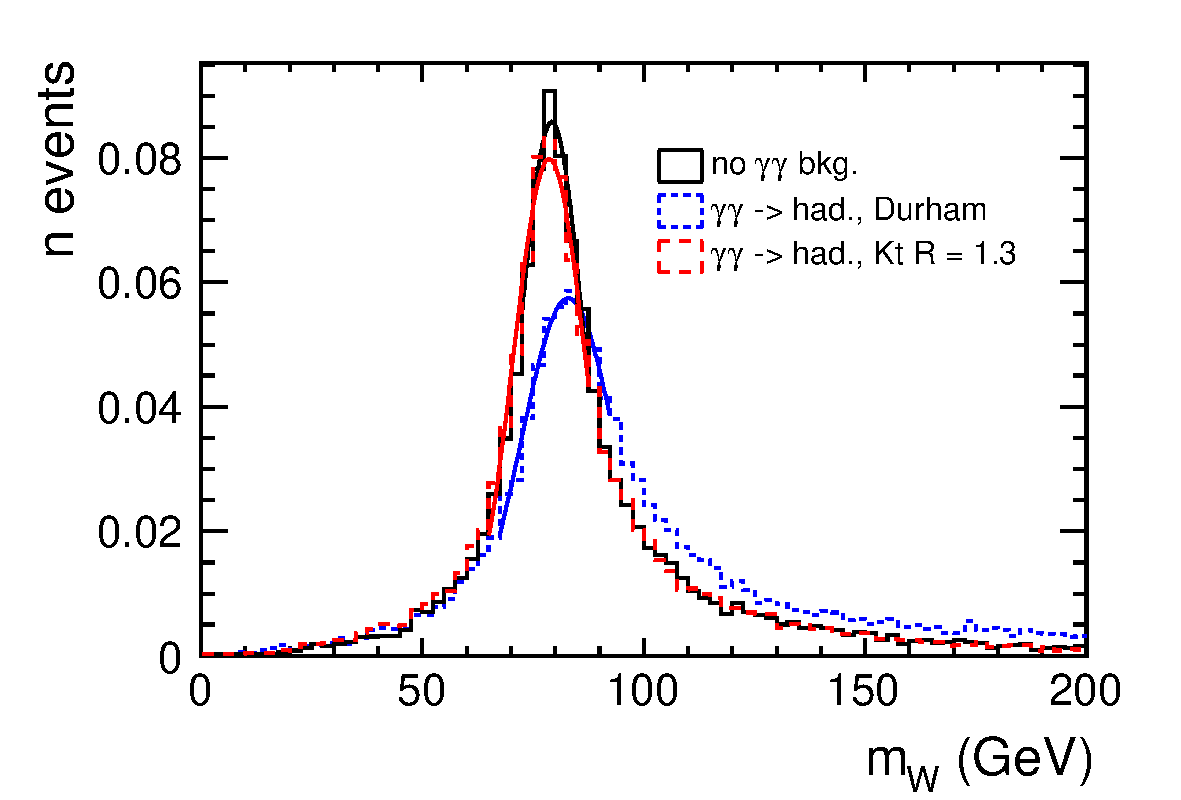
\includegraphics[width=0.95\linewidth]{./chapters/figures/wwjeting.pdf}
		
	\caption{Reconstructed mass of the hadronically decaying $W$ boson at $\sqrt{s}=$1\,TeV without pile-up compared to the situation with pile-up in absence (``Durham'') or presence (``Kt'') of a mitigation strategy in the analysis. From~\cite{Rosca:2016hcq}. 
	}
	\label{fig:WW_overlayremoval}
\end{figure}

Both full-simulation studies used only three out of five possible angular distributions which could provide sensitivity to TGCs: besides the production angle of the $W^-$, the two angles describing the direction of the decay lepton in the restframe of its mother $W$ were considered in a five-parameter fit based on MC templates. The free parameters of the fit were the three TGCs $ g^Z_1$, $\kappa_\gamma$ and $\lambda_\gamma$ as well as the absolute values of the electron and positron beam polarisations. With this approach, statistical uncertainties of about $6$-$7 \cdot 10^{-4}$ were obtained for all three couplings for an integrated luminosity of 500\,fb$^{-1}$ at $\sqrt{s}=$500\,GeV, shared equally between all four beam polarisation configurations.
In the context of the 500\,GeV analysis a thorough evaluation of the systematic errors was performed. It was found at the time that uncertainties on the selection efficiencies of signal and background of 0.2\% and 1\%, respectively, would lead to systematic effects in the same order of magnitude as the statistical uncertainty for 500\,fb$^{-1}$.

A recent study dedicated to a global fit of total and differential cross sections of various SM processes sensitive to TGCs and/or beam polarisation has shown, however, that a much better control of systematic effects can be achieved --- provided that {\em both} beams are polarised~\cite{bib:PhDRobert, Fujii:2018mli}.  

The full simulation study at $\sqrt{s}=$1\,TeV, following the same fitting approach, found statistical uncertainties of about $2$-$3 \cdot 10^{-4}$ for all three TGCs for an integrated luminosity of 1000\,fb$^{-1}$. The effect of different sharings of the luminosity between the four polarisation sign combinations on the TGC precisions were found to be minor. 

\subsubsection{Extrapolation of TGC prospects to 250\,GeV}

While extensive studies of $WW$ production exist at higher center-of-mass energies, no complete analysis based on full detector simulation is available yet for $\sqrt{s}=$250\,GeV. Nevertheless substantial progress has been made in various important aspects which have been incorporated in
an extrapolation~\cite{Fujii:2017vwa} based on a) the previously discussed full-simulation studies at 500\,GeV~\cite{Marchesini:94888} and 1\,TeV~\cite{Rosca:2016hcq} and b) the actual LEP results at $\sim$ 200\,GeV~\cite{Schael:2004tq}:
\begin{itemize}
\item As discussed in Sec.~\ref{subsec:phys_WW}, the sensitivity of measured cross sections to the TGCs depends on the center-of-mass energy as $s/m_W^2$.
\item Naively, the statistical uncertainties on measured cross sections scale as $1/\sqrt{\sigma \L}$. However at higher center-of-mass energies, the $W$ bosons are more and more boosted into the forward direction due to increasing amount of ISR and beamstrahlung. Therefore the experimental acceptance decreases for higher $\sqrt{s}$. A correction factor for this effect has been derived~\cite{Karl:2017let} from a comparison of the full detector simulation studies at 500\,GeV and 1\,TeV.
\item The dependence on the sharing of luminosity between the four different polarisation configurations was found minor~\cite{Rosca:2016hcq} and therefore no corrections for differences in the assumptions of the full simuation studies w.r.t.\ the H20 running scenario (c.f.\ Sec.~\ref{subsec:runscen_pol}) were applied.
\item The improved treatment of systematic uncertainties based on a nuisance parameter technique in a global fit to many observables and datasets explored in~\cite{bib:PhDRobert} was assumed, which leads to a constant ratio between systematic and statistical uncertainties up to luminosities of at least 2\,ab$^{-1}$.
\item The full simulation studies were found to be limited their MC-based, binned fit of 3D-template histograms. The relative improvement expected when including the fully hadronic channel and when exploiting all five sensitive angles (production angle of one of the $W$ bosons plus decay angles of both $W$ bosons, see e.g.\ Fig. 5.16 in~\cite{Marchesini:94888} for an ilustration) in an unbinned fit~\cite{Barklow:1995sk}, or, equivalently, when applying an optimal observable technique~\cite{Diehl:1997ft, Diehl:2002nj}, was estimated in a parton-level study to be a factor 2.4 in the case of $ g^Z_1$, and a factor of 1.9 for the other two couplings.
\item Since none of the ILC full-simulation studies evaluated the precisions for single-coupling fits, i.e.\ when fixing the other two anomalous couplings to 0 as done in hadron collider studies,
the corresponding LEP2 results~\cite{Schael:2004tq} were extrapolated up in center-of-mass energy,
and then the minimum of this extrapolation and of the 3-coupling extrapolation from ILC studies was taken.
\end{itemize}

The results of this procedure are displayed in Tab.~\ref{table:ew_tgc} and Figs~\ref{fig:TGC_1par} and~\ref{fig:TGC_3par} in comparison with the LEP2 and LHC results as well as HL-LHC projections, where applicable. In case of the single-parameter fits, the 250\,GeV stage of the ILC will improve the precision on $ g^Z_1$ and $\kappa_\gamma$ by factors of 5 and 30 w.r.t\ to HL-LHC, while the projections for $\lambda_\gamma$ are comparable. The loss in precision when fitting all three couplings simultaneously to ILC data is minor, and the resulting precisions are used as input for the EFT-based Higgs coupling fit discussed in Sec.~\ref{subsec:higgs_lhcilc}. Actually it has been shown in the past that even the 14 complex couplings in the most general parametrisation of triple gauge boson vertices, including e.g.\ $CP$ violating contributions, can be determined simulataneously at future $e^+e^-$ linear colliders when both beams are polarised and all polarisation configurations, including transverse polarisation, are exploited~\cite{Diehl:2002nj}.

\begin{table}
\begin{center}
  \begin{tabular} {|l|c||c|c|c||c|c|c||}
    \hline
 &   &  \multicolumn{3}{|c||}{total error ($\times 10^{-4}$) } & \multicolumn{3}{c||}{correlation} \\
    \hline
    Exp & $N_{par}$ & $ g^Z_1$  & $\kappa_\gamma$ & $\lambda_\gamma$ & $g^Z_1\ \kappa_\gamma$ &  $g^Z_1\ \lambda_\gamma$  & $\kappa_\gamma\ \lambda_\gamma$  \\
    \hline
    LEP~2     & 3     &  $516$  & $618$  & $376$  & -0.17 & -0.62 & -0.15 \\
    ILC~250   & 3        & $4.4$ & $5.7$ & $4.2$ & 0.63 & 0.48 & 0.35 \\
    \hline
    LEP~2     & 1     & $300$ & $626$ & $292$ & -- & -- & -- \\
    LHC      & 1     & $319$ & $1077$ & $198$ & -- & -- & -- \\
    HL-LHC   & 1      & $19$ & $160$ & $4$ & -- & -- & -- \\
    ILC~250   & 1       & $3.7$ & $5.7$ & $3.7$ & -- & -- & -- \\
    \hline

\end{tabular}
  \caption{TGC precisions for LEP~2, Run1 at LHC, HL-LHC and the ILC at $\sqrt{s}=250$~GeV with 2000~fb$^{-1}$ luminosity (ILC~250). The LEP~2 result is from ALEPH~\cite{Schael:2004tq} at  $\sqrt{s}\approx 200$~ GeV with
    0.68~fb$^{-1}$.  The LHC result is from ATLAS\cite{Aad:2014mda} at $\sqrt{s}=7$~TeV with 4.6~fb$^{-1}$.  The HL-LHC estimate is from a 2013 overview of HL-LHC physics~\cite{bib:HLLHCMoenig}. From~\cite{Fujii:2017vwa}.}
\label{table:ew_tgc}
\end{center}
\end{table}

\begin{figure}
	\centering
		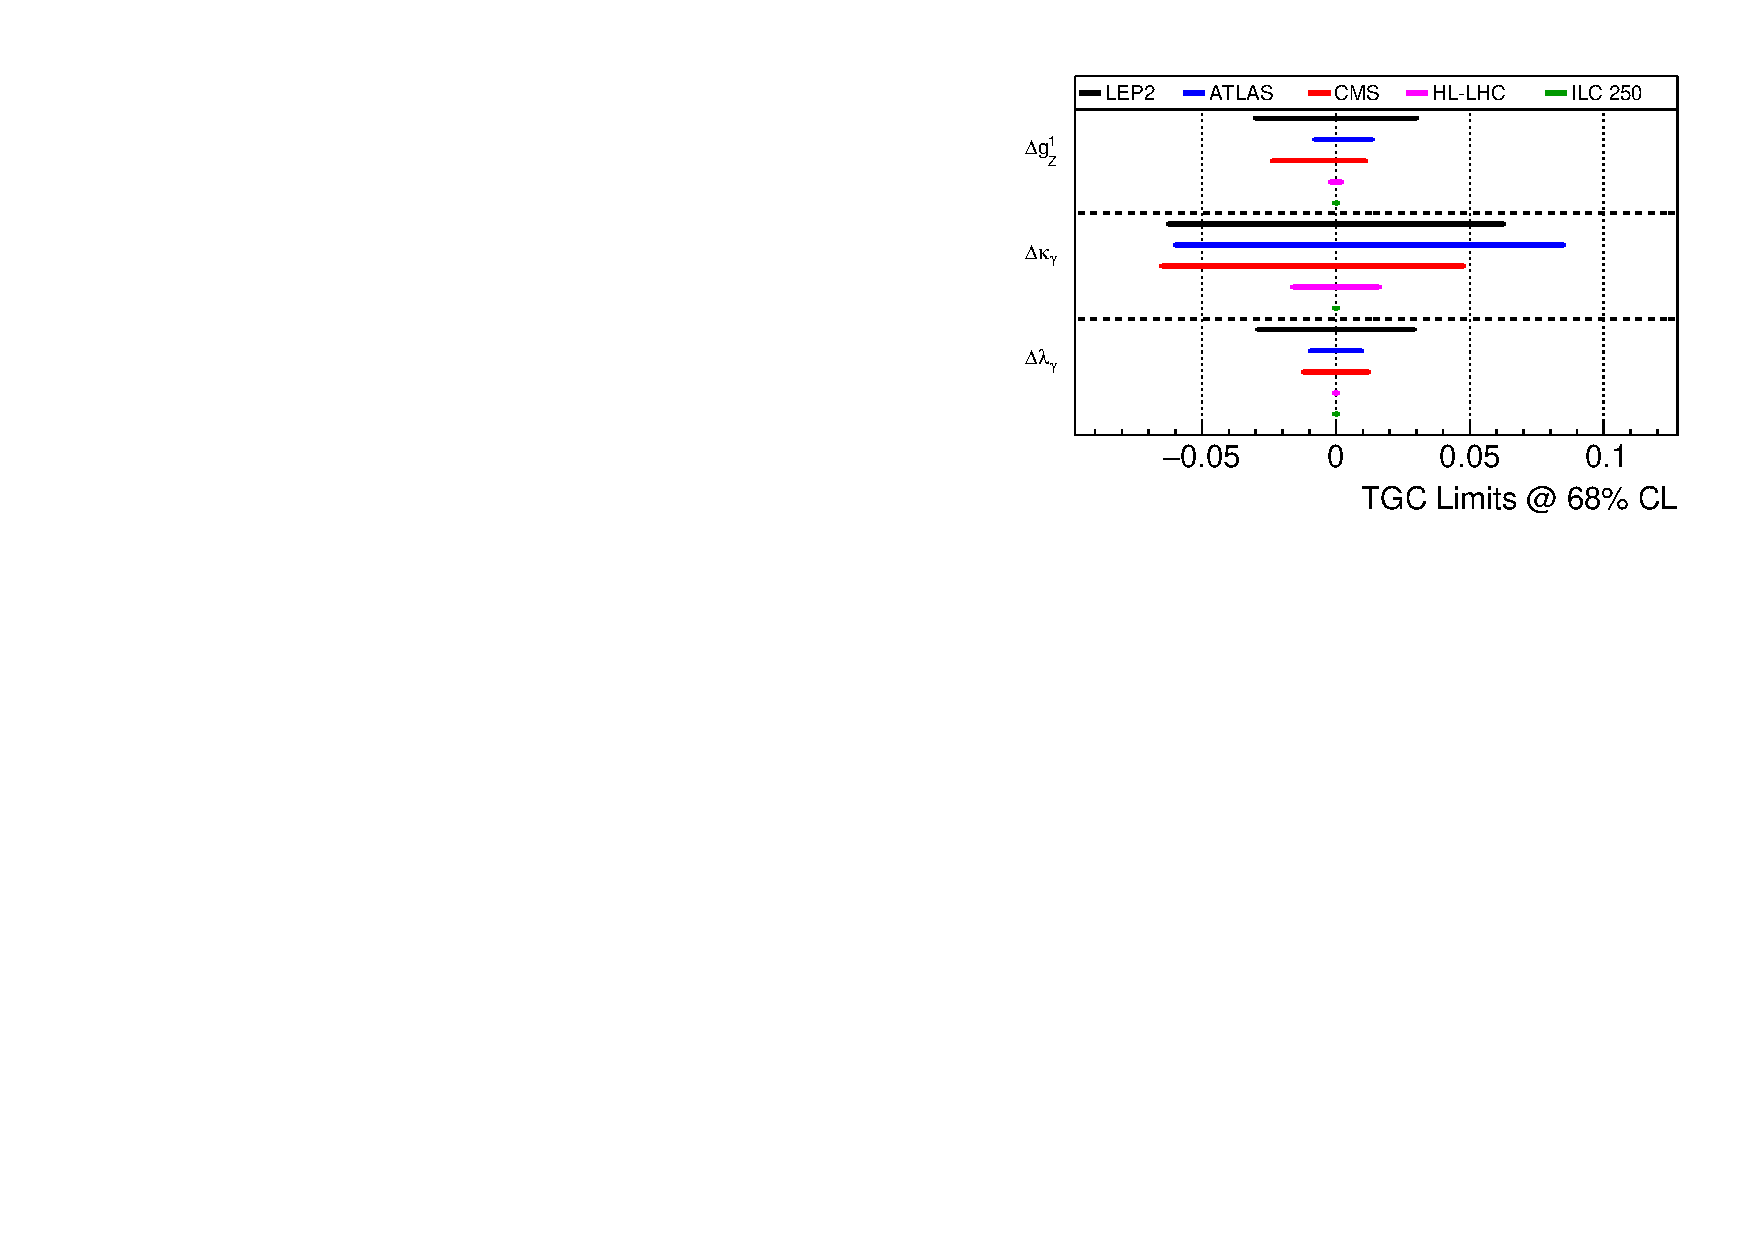
\includegraphics[width=0.95\linewidth]{./chapters/figures/TGC_LHCsep.pdf}
		
	\caption{Comparison of the reachable TGC precision from single parameter fits: ILC~\cite{bib:TGC_EPS17}, final results from LEP combined from ALEPH, L3 and OPAL results~\cite{bib:LEPTGC} and the LHC TGC limits for $\sqrt{s} = 8$\,TeV data and an integrated luminosity of $\mathcal{L} = 20.3$\ifb and  $\mathcal{L} = 19.4$\ifb for ATLAS and CMS, respectively~\cite{bib:LHCTGC}. 
	}
	\label{fig:TGC_1par}
\end{figure}

\begin{figure}
	\centering
		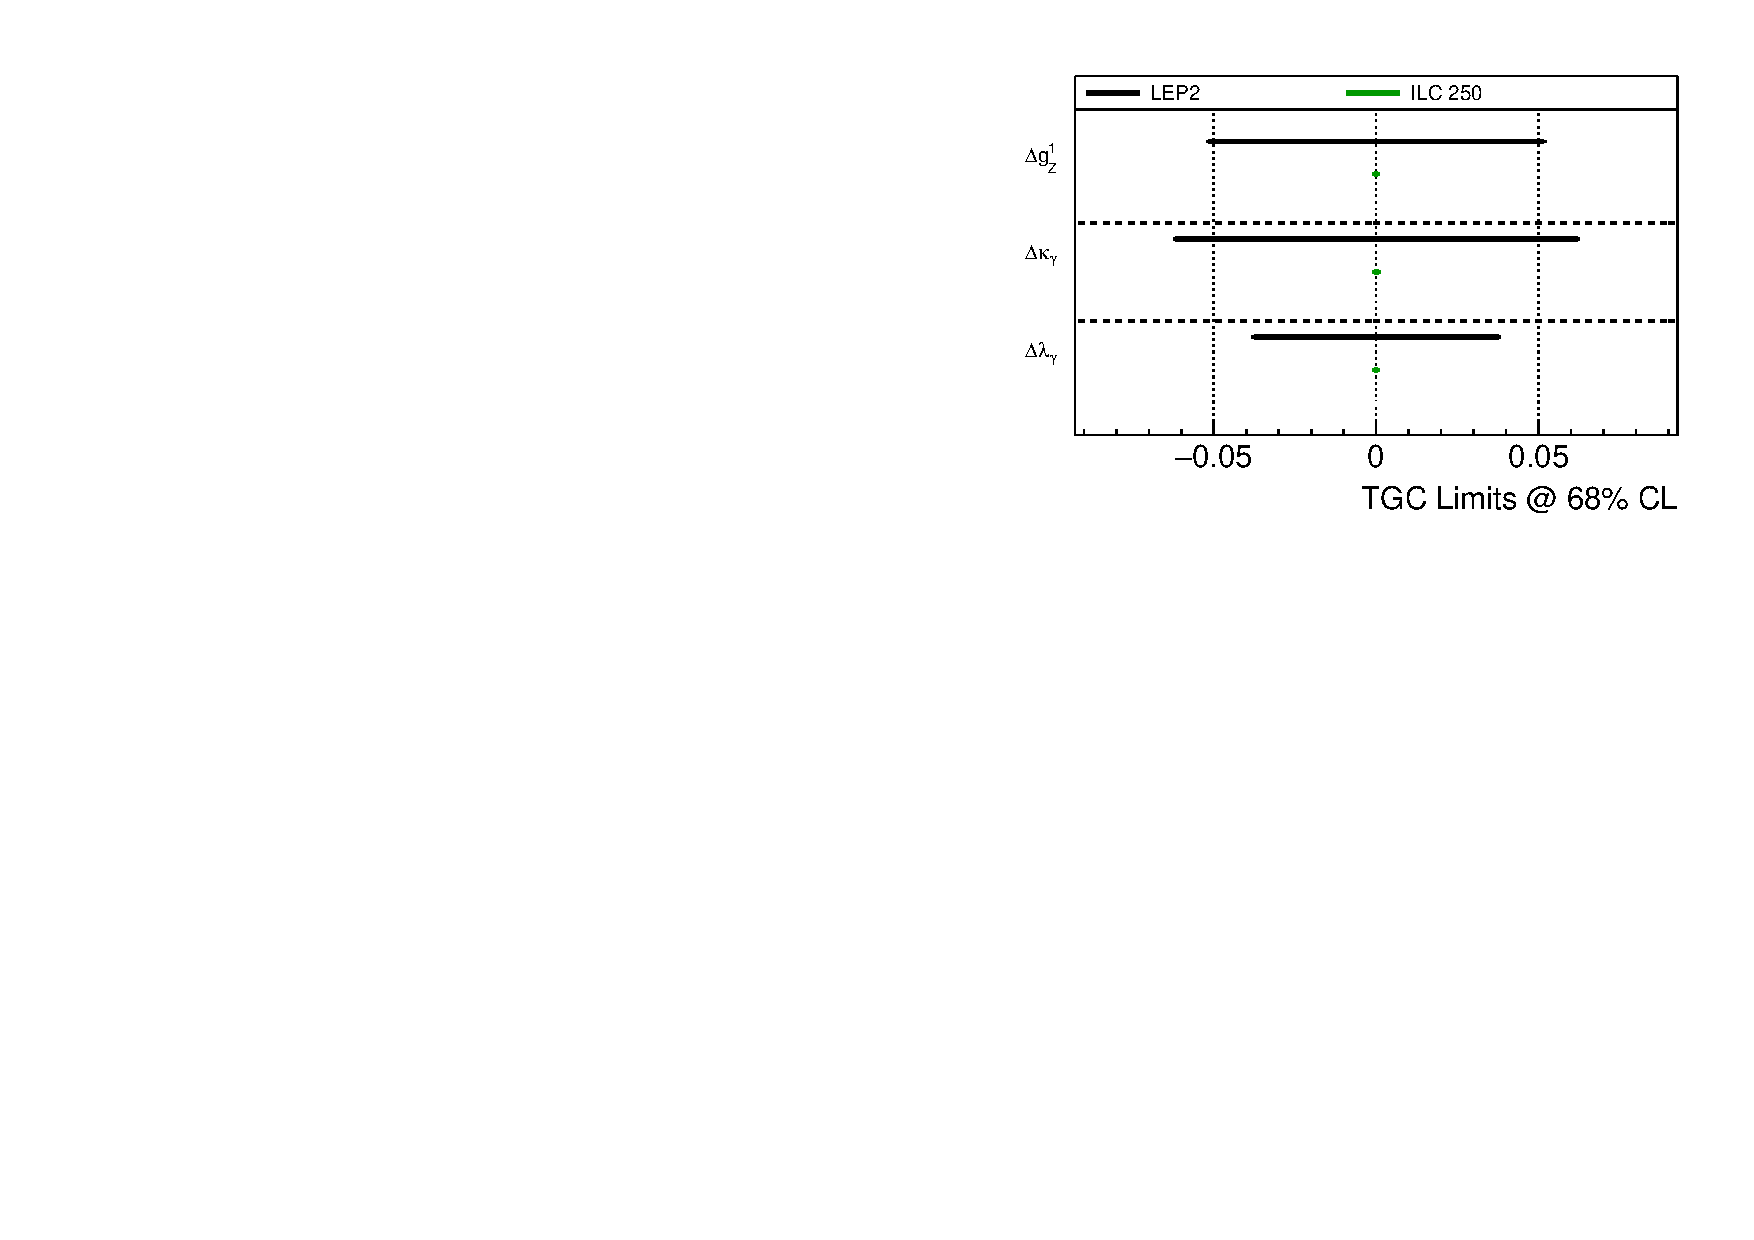
\includegraphics[width=0.95\linewidth]{./chapters/figures/TGC_Multi.pdf}
		
	\caption{Comparison of the reachable TGC precision from a simultaneous fit of all three parameters: ILC~\cite{bib:TGC_EPS17} and final results from LEP combined from ALEPH, L3 and OPAL results~\cite{bib:LEPTGC}. No comparable hadron collider results are available.
	}
	\label{fig:TGC_3par}
\end{figure}

\subsubsection{$W$ Mass Measurement at 250\,GeV}
\label{subsubsec:ew_mw}
The analysis of $W^+W^- \to qql\nu$ discussed in the previous sections, as well as the study of single-$W$ events also offer an excellent setting for the measurement of the $W$ mass. As discussed in Sec.~\ref{subsec:phys_ff}, the available statistics at the 250\,GeV ILC will be about a factor of 2000 larger than at LEP2, which makes it obvious that a pure consideration of statistical uncertainties is meaningless. While the studies discussed in Sec.~\ref{subsubsec:ew_fullsimww} showed that this kind of events can be selected with high efficiency and purity, a careful extrapolation of the systematic uncertainties of previous measurements is therefore much more instructive than the evaluation of the statistical uncertainty from full detector simulation.
Apart from a scan of the production threshold, kinematic reconstruction of $W$ pair events 
and calorimetric comparison of hadronic $W$ and  $Z$ decays in single-boson events are the most promising techniques, which are described in detail in~\cite{Freitas:2013xga, Wilson:2016tto}.   With a combination of methods and considering advances in theory as well as in the performance of the detectors the systematic limit has been estimated as 2.4\,MeV. This is expected to be reached already at the 250\,GeV stage of the ILC. Additional datasets at higher center-of-mass energies 
could then provide independent information in order to cross-check and constrain systematic effects.
